% $Header$

\documentclass{beamer}

% Copyright 2004 by Till Tantau <tantau@users.sourceforge.net>.
%
% In principle, this file can be redistributed and/or modified under
% the terms of the GNU Public License, version 2.
%
% However, this file is supposed to be a template to be modified
% for your own needs. For this reason, if you use this file as a
% template and not specifically distribute it as part of a another
% package/program, I grant the extra permission to freely copy and
% modify this file as you see fit and even to delete this copyright
% notice. 


\mode<presentation>
{
	\usetheme{Madrid}
	
	%\setbeamercovered{transparent}
	% or whatever (possibly just delete it)
}


\usepackage[english]{babel}
% or whatever

\usepackage[latin1]{inputenc}
% or whatever

\usepackage{times}
\usepackage[T1]{fontenc}
\graphicspath{ {./graphics/} }
\usepackage{amsthm}

\newtheorem*{remark}{Remark}
\newtheorem*{prop}{Proposition}
\newtheorem*{proofnosq}{Proof.}


\title[Analyzing Snapshot Isolation] % (optional, use only with long paper titles)
{Analyzing Snapshot Isolation}

\author[Andrea Cerone, Alexey Gotsman] % (optional, use only with lots of authors)
{\textit{Andrea Cerone \and Alexey Gotsman \\ \footnotesize presented by Dima Kuznetsov}}



\institute[IMDEA] % (optional, but mostly needed)
{IMDEA Software Institute}

\date[PODC 2016] % (optional, should be abbreviation of conference name)
{PODC 2016}

\subject{Theoretical Computer Science}
% This is only inserted into the PDF information catalog. Can be left
% out. 


% If you have a file called "university-logo-filename.xxx", where xxx
% is a graphic format that can be processed by latex or pdflatex,
% resp., then you can add a logo as follows:

% \pgfdeclareimage[height=0.5cm]{university-logo}{university-logo-filename}
% \logo{\pgfuseimage{university-logo}}



% Delete this, if you do not want the table of contents to pop up at
% the beginning of each subsection:
\AtBeginSubsection[]
{
	\begin{frame}<beamer>{Outline}
	    \tableofcontents[currentsection,currentsubsection]
    \end{frame}
}


% If you wish to uncover everything in a step-wise fashion, uncomment
% the following command: 

%\beamerdefaultoverlayspecification{<+->}


\begin{document}

\begin{frame}
	\titlepage
\end{frame}

\begin{frame}{Outline}
	\tableofcontents
\end{frame}

\section{Introduction}

\begin{frame}{Intro}
	\begin{itemize}
		\item We focus on \emph{Snapshot Isolation} presented in the last talk
		\item ... same context of DBMS and transactional memory systems
	\end{itemize}
\end{frame}

\begin{frame}{Intro}
	\begin{itemize}
		\item DBMS typically offer various guarantees for transaction management
		\item Each mode exhibits different \emph{anomalies}
		\item Stronger modes exhibit less anomalies at expense of performance
		\begin{itemize}
			\item Stronger guarantees incur more overhead on the DBMS side
			\item Less allowed behaviors $ \rightarrow $ more concurrent transactions expected to abort
		\end{itemize}
	\end{itemize}
\end{frame}

\begin{frame}{Snapshot Isolation}
	FIXME
	\textbf{Snapshot Isolation} - originally specified as operational model:
	\begin{itemize}
		\item When transaction $ T $ begins, $ snapshot_T $ is taken
		\item All reads in $ T $ read values from $ snapshot_T $
		\item All writes in $ T $ write to transient write-set
		\item T commits only if passes write conflict check:
		\begin{itemize}
			\item No object in $T$'s write-set was updated by other transactions since $snapshot_T$ was taken
		\end{itemize}
	\end{itemize}	
\end{frame}

%\begin{frame}{Example}
%	The operational model allows write-skew anomalies
%	\begin{figure}
%		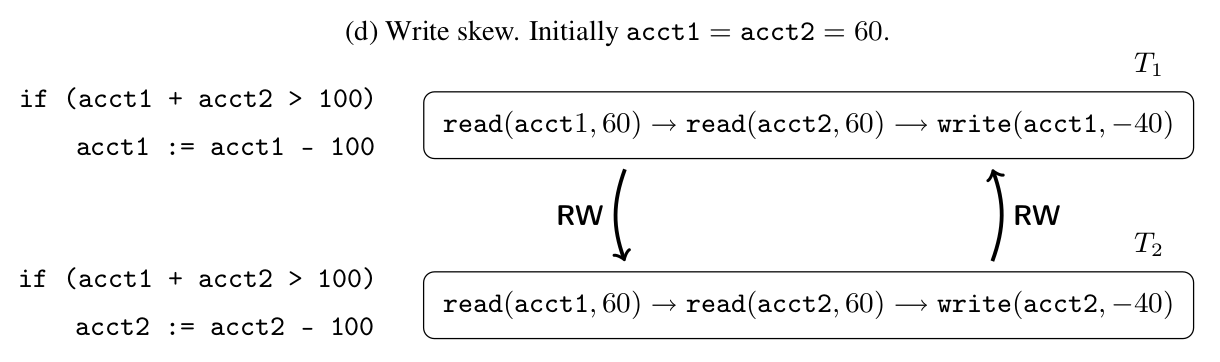
\includegraphics[scale=0.22]{write-skew}
%	\end{figure}
%\end{frame}


\section{Snapshot Isolation}
\subsection{Definitions}
\begin{frame}{Definitions}
	We'll start by formulating a declarative definition of Snapshot Isolation.
\end{frame}

\begin{frame}
	We'll use a lot of notation similar to Daniel's talk two weeks ago
	\begin{itemize}
		\item $ Obj =  \{ x, y, \dots \} $ - objects in the data-set
		\item $ Event = \{ e, f, \dots \} $ - transaction events
		\item $ Op = \{ read(x,n), write(x, n) \mid x \in Obj, n \in \mathbb{Z}\} $ 
		\item $ op: Event \rightarrow Op $
	\end{itemize}
\end{frame}

\begin{frame}
	\begin{definition}
		A \textbf{transaction} $ T, S, \dots $ is a pair $ (E, po ) $ where $ E \subseteq Event $ is a \emph{finite}, non-empty set of events and \textbf{program-order} $ po \subseteq E \times E $ is a total order.
	\end{definition}
	Where ...
	\begin{itemize}
		\item \textit{total order} is a transitive and irreflexive relation that orders all pairs
	\end{itemize}
\end{frame}

\begin{frame}
	\begin{definition}
		A \textbf{history} is a pair $ \mathcal{H} = (\mathcal{T},SO) $ where $\mathcal{T}$ is a finite set of transactions with disjoint set of events and the \textbf{session-order} $ SO \subseteq \mathcal{T} \times \mathcal{T} $ is a union of total orders defined on disjoint subsets of $\mathcal{T}$, which correspond to transactions in different sessions.
	\end{definition}
\end{frame}

\begin{frame}
	We elide treatment of:
	\begin{itemize}
		\item aborted transactions - all transactions in any history are committed.
		\item infinite computations - histories are always finite.
	\end{itemize}
\end{frame}

\begin{frame}
	\begin{definition}
		An \textbf{abstract execution} is a tuple $ \mathcal{X} = (\mathcal{T}, SO, VIS, CO) $, where $(\mathcal{T}, SO)$ is a history and the \textbf{visibility} and \textbf{commit order} $ VIS, CO \subseteq \mathcal{T} \times \mathcal{T} $ are such that $ VIS \subseteq CO $ and $CO$ is total.
	\end{definition}
\end{frame}

\begin{frame}
	\begin{itemize}
		\item We'll use $ (T, S) \in VIS$ and $ T \overset{VIS}{\longrightarrow} S $ interchangeably for $VIS$ and other relations.
		\item For $\mathcal{H}=(\mathcal{T}, SO)$ we'll shorten $(\mathcal{T}, SO, VIS, CO)$ to $(\mathcal{H}, VIS, CO)$
	\end{itemize}
\end{frame}

\begin{frame}
	For the relations defined in abstract execution:
	\begin{itemize}
		\item $ T \overset{VIS}{\longrightarrow} S $ means that $T$ is included in $S$'s snapshot.
		\item $ T \overset{CO}{\longrightarrow} S $ means that $T$ is committed before $S$.
		\item $ VIS \subseteq CO $ makes sure that snapshots include only already committed transactions.
	\end{itemize}
\end{frame}

\begin{frame}
	For a set $ A $ and a total order $ R \subseteq A \times A $
	\begin{itemize}
		\item $max_R(A) = \{ a \mid \forall b \in A: a = b \vee (b, a) \in R \} $
		\item $min_R(A) = \{ a \mid \forall b \in A: a = b \vee (a, b) \in R \} $
	\end{itemize}
\end{frame}

\begin{frame}
	For $T = (E, po)$ we'll use:
	\begin{itemize}
		\item $ T \vdash write(x,n) $ if $T$ writes to $x$ and $n$ is s.t.
		$$ op\left(max_{po}\{e \mid op\left(e\right)  = write\left(x, \_ \right) \} \right) = write(x,n)$$
		\item $ T \vdash read(x,n) $ if $T$ reads $x$ before writing to is and $n$ is s.t.
		$$ op\left(min_{po}\{e \mid op\left(e\right)  = \_\left(x, \_ \right) \} \right) = read(x,n)$$
	\end{itemize}
	We'll also use $ WriteTx_x = \{ T \mid T \vdash write(x,\_)\}$
\end{frame}

\begin{frame}
	We'll now try to define \emph{snapshot isolation} and \emph{serializability} in terms of \textbf{consistency axioms}:
	\begin{equation*}
		\begin{aligned}
			ExecSI = {} &
				\begin{aligned} 
					\{ \mathcal{X} \mid \mathcal{X} \vDash & \textsc{Int} \wedge \textsc{Ext} \wedge \textsc{Session} \wedge \\
														& \textsc{Prefix} \wedge \textsc{NoConflict} \}
				\end{aligned}
				\\
			ExecSER = {} & \{ \mathcal{X} \mid \mathcal{X} \vDash \textsc{Int} \wedge \textsc{Ext} \wedge \textsc{Session} \wedge \textsc{TotalVis} \} \\
			HistSI = {} & \{ \mathcal{H} \mid \exists VIS,CO : (\mathcal{H}, VIS, CO) \in ExecSI \} \\
			HistSER = {} & \{ \mathcal{H} \mid \exists VIS,CO : (\mathcal{H}, VIS, CO) \in ExecSER \} 
		\end{aligned}
	\end{equation*}
\end{frame}

\begin{frame}
	\begin{definition}[Internal consistency]
		\textsc{Int} - ensures that a read event $e$ on object $x$ returns the same value a as the last write or read on $x$ in the same transaction.
		\begin{multline*}
			\forall (E,po)\in \mathcal{T} . \forall e \in E . \forall x,n: \\
				op(e) = read(x,n) \wedge \{f\mid op(f) = \_(x,\_)\wedge f \overset{po}{\longrightarrow} e\} \ne \emptyset \Rightarrow \\
				op\left(max_{po}\{f \mid op\left(f\right) = \_ \left(x, \_\right) \wedge f \overset{po}{\longrightarrow} e\}\right) = \_(x,n)
		\end{multline*}
	\end{definition}
\end{frame}

\begin{frame}
	\begin{definition}[External consistency]
		\textsc{Ext} - ensures that if $T\vdash read(x,n)$ then the value is taken from the last visible transaction that wrote to $x$ according to commit order.
		\begin{multline*}
			\forall T \in \mathcal{T} . \forall x, n: \\
			T \vdash read(x,n) \Rightarrow
			max_{CO}\left( VIS^{-1}\left( T \right) \cap WriteTx_x \right) \vdash write(x,n)
		\end{multline*}
	\end{definition}
	Where ...
	\begin{itemize}
		\item $R^{-1}(a) = \{ b \mid (b, a) \in R \}$
	\end{itemize}
\end{frame}

\begin{frame}
	\begin{definition}[Session visibility]
		\textsc{Session} - requires a snapshot to include all preceding transactions of the same session.
		$$ SO \subseteq VIS $$
	\end{definition}
\end{frame}

\begin{frame}
	\begin{figure}
		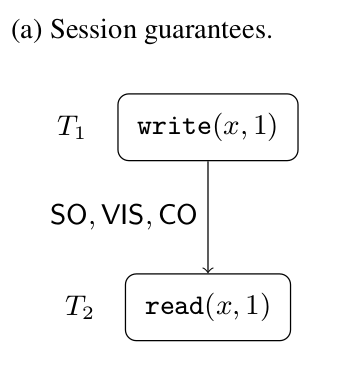
\includegraphics[scale=0.3]{fig2a}
	\end{figure}
\end{frame}

\begin{frame}
	\begin{definition}[Prefix]
		\textsc{Prefix} - ensures that if snapshot taken by $T$ includes $S$, then it includes all transactions committed before $S$ as well.
		$$ CO; VIS \subseteq VIS $$
	\end{definition}
	Where ...
	\begin{itemize}
		\item $R_1;R_2 = \{(a,b) \mid \exists c: (a,c) \in R_1 \wedge (c,b) \in R_2\} $
	\end{itemize}
\end{frame}

\begin{frame}
	The \textbf{long-fork} anomaly is prevented by \textsc{Prefix} axiom:
	\begin{figure}
		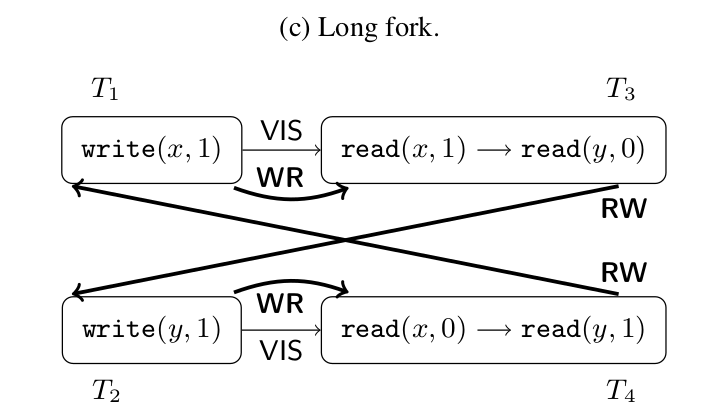
\includegraphics[scale=0.3]{fig2c}
	\end{figure}
\end{frame}

\begin{frame}
	\begin{definition}[No conflict check]
		\textsc{NoConflict} - ensures that for any two transactions writing to the same object, one has to be aware of the other.
		\begin{multline*}
		\forall T,S \in \mathcal{T}. \forall x,n . \\
		\left( T,S \in WriteTx_x \wedge T \ne S \right)
		\Rightarrow
		\left( T \overset{VIS}{\longrightarrow} S \vee S \overset{VIS}{\longrightarrow} T \right)
		\end{multline*}
	\end{definition}
\end{frame}

\begin{frame}
	The \textbf{lost-update} anomaly is prevented by \textsc{NoConflict} axiom:
	\begin{figure}
		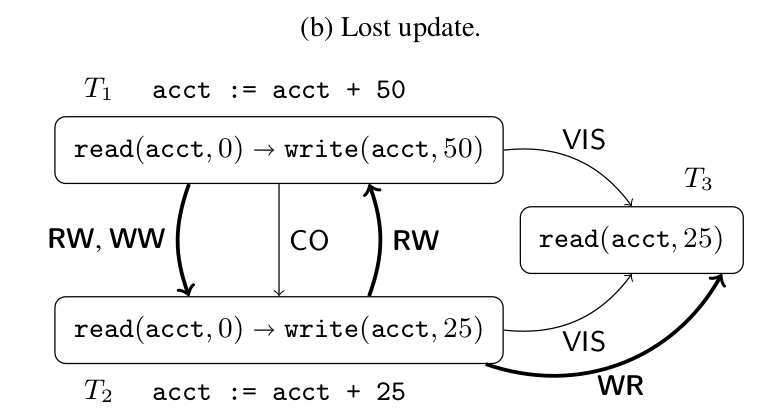
\includegraphics[scale=0.3]{fig2b}
	\end{figure}
\end{frame}

\begin{frame}
	\begin{definition}[Total visibility]
		\textsc{TotalVis} - requires total order on the visibility relation, giving us \emph{serializability} of transactions.
		$$ VIS = CO $$
	\end{definition}
\end{frame}

\begin{frame}
	The \textbf{write-skew} anomaly allowed by Snapshot Isolation is prevented by \textsc{TotalVis} axiom:
	\begin{figure}
		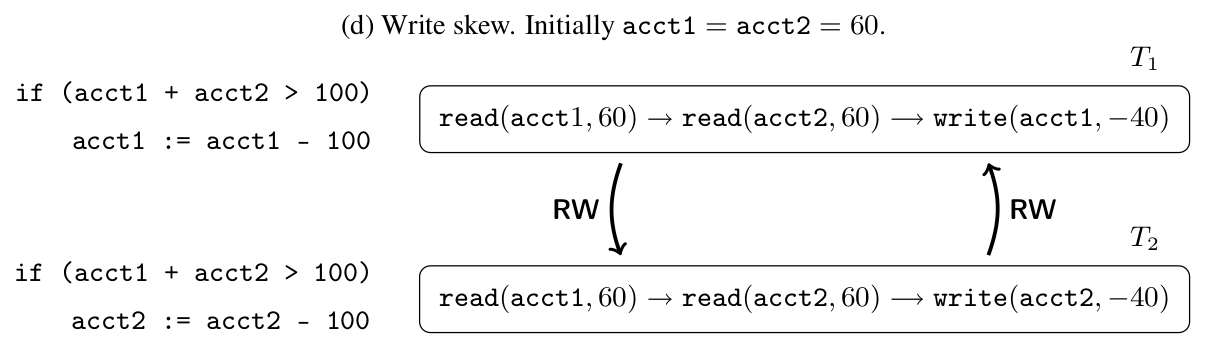
\includegraphics[scale=0.25]{fig2d}
	\end{figure}
\end{frame}

\subsection{Dependency Graphs}

\begin{frame}
	\begin{itemize}
		\item Our goal now is to characterize SI in terms of dependencies between transactions.
		\item Then we'll be able to decide whether SI allows a given history by looking for appropriate dependencies.
	\end{itemize}
\end{frame}

\begin{frame}
	\begin{definition}
		Consider execution $\mathcal{X} = (\mathcal{T}, SO, VIS, CO)$, for $x \in Obj$ we define \textbf{read-dependency} $WR_\mathcal{X}(x)$ over $\mathcal{T}_\mathcal{X}$ as:
		\begin{multline*}
			T \xrightarrow{WR_\mathcal{X}(x)} S \Leftrightarrow \\
			S \vdash read(x,n) \wedge T = max_{CO}\left( VIS^{-1}(S) \cap WriteTx_x \right)
		\end{multline*}
	\end{definition}
	Informally: T $ \xrightarrow{WR_\mathcal{X}(x)} S $ means that $S$ reads $T$'s write to $x$.
\end{frame}

\begin{frame}
	\begin{definition}
		Consider execution $\mathcal{X} = (\mathcal{T}, SO, VIS, CO)$, for $x \in Obj$ we define \textbf{write-dependency} $WW_\mathcal{X}(x)$ over $\mathcal{T}_\mathcal{X}$ as:
		$$
			T \xrightarrow{WW_\mathcal{X}(x)} S \Leftrightarrow T \xrightarrow{CO}S \wedge T,S \in WriteTx_x
		$$
	\end{definition}
	Informally: T $ \xrightarrow{WW_\mathcal{X}(x)} S $ means that $S$ overwrites $T$'s write to $x$.
\end{frame}


\begin{frame}
	\begin{definition}
		Consider execution $\mathcal{X} = (\mathcal{T}, SO, VIS, CO)$, for $x \in Obj$ we define \textbf{anti-dependency} $RW_\mathcal{X}(x)$ over $\mathcal{T}_\mathcal{X}$ as:
		\begin{multline*}
			T \xrightarrow{RW_\mathcal{X}(x)} S \Leftrightarrow \\
			T \ne S \wedge \exists T^\prime . T^\prime \xrightarrow{WR_\mathcal{X}(x)}T \wedge T^\prime \xrightarrow{WW_\mathcal{X}(x)}S
		\end{multline*}
	\end{definition}
	Informally: T $ \xrightarrow{RW_\mathcal{X}(x)} S $ means that $S$ overwrites the write to $x$ read by $T$.
\end{frame}

\begin{frame}
	FIXME add example
\end{frame}

\begin{frame}
	\begin{definition}
		A \textbf{dependency graph} is a tuple $\mathcal{G} = (\mathcal{T}, SO, WR, WW, RW)$, where $(\mathcal{T}, SO)$ is a history and:
		\begin{itemize}
			\item WR: $Obj \rightarrow 2^{\mathcal{T} \times \mathcal{T}}$ is such that:
			\begin{itemize}
				\item $\forall T,S. \forall x . T \xrightarrow{WR(x)}S \Rightarrow $ 
					  $	\exists n. T \ne S \wedge T \vdash write(x,n) \wedge S \vdash read(x,n)$
				\item $\forall S \in \mathcal{T}. \forall x. S \vdash read(x,\_) \Rightarrow \exists T. T \xrightarrow{WR(x)} S $
				\item $\forall T, T^\prime, S \in \mathcal{T}. \forall x. \left( T \xrightarrow{WR(x)} S \wedge T^\prime \xrightarrow{WR(x)} S \right) \Rightarrow T = T^\prime $
			\end{itemize}
		\item WW: $Obj \rightarrow 2^{\mathcal{T} \times \mathcal{T}}$ is such that for every $x \in Obj$, $WW(x)$ is a total order on the set $WriteTx_x$.
		\item RW: $Obj \rightarrow 2^{\mathcal{T} \times \mathcal{T}}$ is derived from WR and WW as in the definition of $WR_\mathcal{X}(x)$.
		\end{itemize}
	\end{definition}
\end{frame}


\begin{frame}
	\begin{prop}
		For any $\mathcal{X} \in ExecSI$,
		$$
			graph(\mathcal{X}) = (\mathcal{T}_\mathcal{X}, SO_\mathcal{X}, WR_\mathcal{X}, WW_\mathcal{X}, RW_\mathcal{X})
		$$
		is a dependency graph.
	\end{prop}
	\begin{proofnosq}
		By showing $graph(\mathcal{X})$ satisfies all requirements of a dependency graph.
	\end{proofnosq}
\end{frame}

\subsection{Characterization}

\begin{frame}
	We'll show that SI is characterized by dependency graphs that contain only cycles with at least two adjacent anti-dependency edges.
\end{frame}

\begin{frame}
	\begin{theorem}
		Let
		$$
		\begin{aligned}
			GraphSER = \{ \mathcal{G} \mid & \left( \mathcal{T}_\mathcal{G} \vDash \textsc{Int} \right) \\
			      & \left(
		      		\left(
		    	  	 SO_\mathcal{G} \cup WR_\mathcal{G} \cup WW_\mathcal{G} \cup RW_\mathcal{G}
			      	\right) \text{is acyclic}
			        \right) \}
		\end{aligned}
		$$
		Then 
		$$
		\begin{aligned}
			HistSER = \{ \mathcal{H} \mid & \exists WR, WW, RW. \\
			& \left( \mathcal{H}, WR, WW, RW \right) \in GraphSER \}
		\end{aligned}
		$$	
	\end{theorem}
	In other words, execution is serializable if it can be extended into an acyclic dependency graph.
\end{frame}


\begin{frame}
	\begin{theorem}
		Let
		$$
			\begin{aligned}
			GraphSI = 
				\{ 
					\mathcal{G} 
					\mid &
					\left( \mathcal{T}_\mathcal{G} \vDash \textsc{Int} \right) \wedge \\
						 & \left(
							\left(
								\left(
									SO_\mathcal{G} \cup WR_\mathcal{G} \cup WW_\mathcal{G}
								\right)  ; RW_\mathcal{G}^?
						\right) \ is \ acyclic
					\right)
				\}	
			\end{aligned}
		$$
		Then
		$$
			HistSI = \{ \mathcal{H} \mid \exists WR, WW, RW. (\mathcal{H}, WR, WW, RW) \in GraphSI \}
		$$
	\end{theorem}
	Where ...
	\begin{itemize}
		\item $R^? = R \cup \{ (a, a) \mid a \in A \}$
	\end{itemize}
\end{frame}


\begin{frame}
Example:
\begin{figure}
	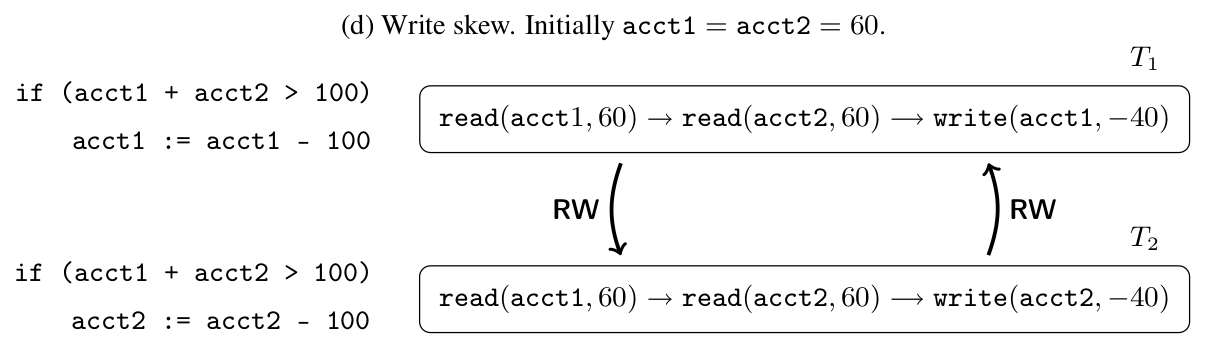
\includegraphics[scale=0.25]{fig2d}
\end{figure}
\begin{itemize}
	\item Prohibited under \textbf{serializability}, and has a dependency graph cycle $ T_1 \xrightarrow{RW} T_2 \xrightarrow{RW} T_1 $.
	\item However, allowed under \textbf{SI}
\end{itemize}
\end{frame}

\begin{frame}
In contrast, following is \emph{not} allowed under SI:
\begin{figure}
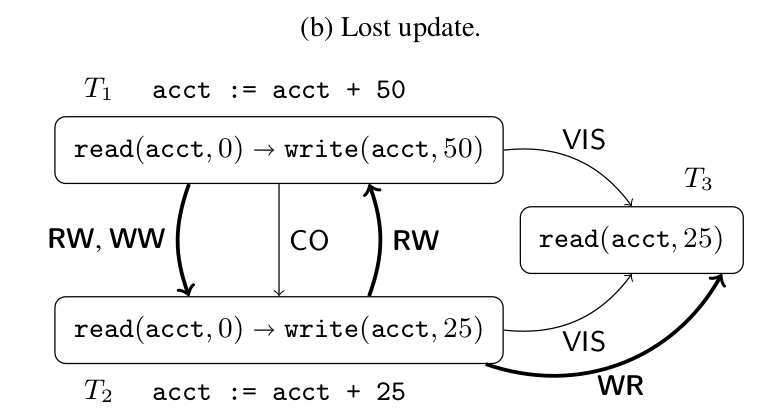
\includegraphics[scale=0.2]{fig2b}
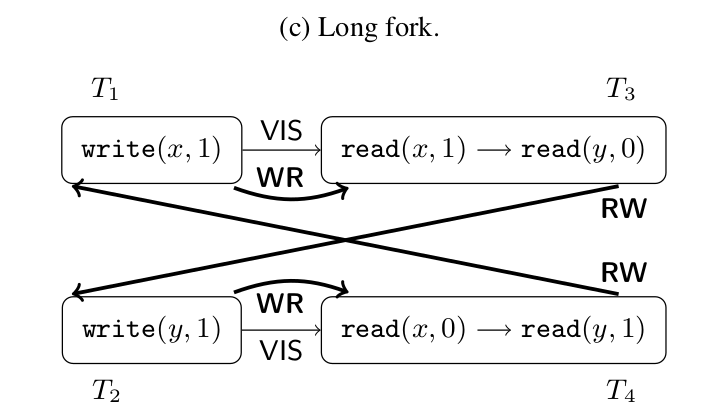
\includegraphics[scale=0.2]{fig2c}
\end{figure}
contain cycles without adjacent anti dependencies.
\end{frame}

\begin{frame}
	To prove it we'll show a stronger result: \\
	\begin{enumerate}
		\item \textbf{Soundness:} $ \forall \mathcal{G} \in GraphSI. \exists \mathcal{X} \in ExecSI. graph(\mathcal{X}) = \mathcal{G} $ 
		\item \textbf{Completeness:} $ \forall \mathcal{X} \in ExecSI. graph(\mathcal{X}) \in GraphSI$
	\end{enumerate}
	The \textit{completeness} closely follows from existing results\footnote{Making Snapshot Isolation Serializable, 2005, A. Fekete et al}. We will focus on the \textit{soundness}.
	
\end{frame}

\begin{frame}
Proof sketch: \\

\begin{itemize}
	\item Construct a basic \textbf{pre-execution} from $\mathcal{G}$
	\item Iteratively extend it until satisfies execution definition
\end{itemize}

\end{frame}

\begin{frame}
	\begin{definition}
		A tuple $\mathcal{P} = (\mathcal{T}, SO, VIS, CO) $ is a \textbf{pre-execution} if it satisfies all the conditions of being an \emph{execution}, except $CO$ is a \textit{strict partial order} that may not be total.
	\end{definition}
	\begin{definition}
		We let $PreExecSI$ be the set of pre-executions satisfying the SI axioms:
		$$
			\begin{aligned}
				PreExecSI = \{ \mathcal{P} \mid \mathcal{P} \vDash & INT \wedge EXT \wedge SESSION \wedge \\
																   & PREFIX \wedge NOCONFLICT \}
			\end{aligned}
		$$
	\end{definition}
	Where ...
	\begin{itemize}
		\item \textit{strict partial order} is a transitive and irreflexive relation
	\end{itemize}
\end{frame}

\begin{frame}
	\begin{itemize}
		\item For a given dep. graph $\mathcal{G} = (\mathcal{H}, WR, WW, RW)$, let $\mathcal{P} = (\mathcal{H}, VIS, CO)$ a respective pre-execution.
		\item To conform with $\mathcal{G}$ we require that $VIS,CO$ hold: \\
			\begin{align}
				SO \cup WR \cup WW & \subseteq VIS \\
				CO; VIS & \subseteq VIS \\
				VIS & \subseteq CO \\
				CO; CO & \subseteq CO \\
				VIS; RW & \subseteq CO
			\end{align}
	\end{itemize}
\end{frame}

\begin{frame}
	\begin{lemma}
		Let $\mathcal{G} = (\mathcal{T}, SO, WR, WW, RW)$ be a dependency graph, for any relation $R \subseteq \mathcal{T} \times \mathcal{T}$, the relations
		$$
			\begin{aligned}
				VIS = {} & (((SO \cup WR \cup WW); RW^?) \cup R)^*; \\
				         & (SO \cup WR \cup WW) \\
				 CO = {} & (((SO \cup WR \cup WW); RW^?) \cup R)^+
			\end{aligned}
		$$
		are a solution to the system of inequalities in the previous slide. They also are the smallest solution to the system for which $R \subseteq CO$.
	\end{lemma}
	Where... 
	\begin{itemize}
		\item $R^+$ a transitive closure of $R$
		\item $R^*$ a transitive and reflexive closure of $R$
	\end{itemize}
\end{frame}

\begin{frame}
	FIXME add intuition
\end{frame}

\begin{frame}
	\begin{proof}
		Let $\mathcal{G} = (\mathcal{T}, SO, WR, WW, RW) \in GraphSI$
		\begin{itemize}
			\item Define $\mathcal{P}_0$ derived from the last lemma by fixing $R_0 = \emptyset$.
			\item Construct $\{\mathcal{P}_i = (\mathcal{T}, SO, VIS_i, CO_i)\}^n_{i=0}$ series of pre-executions.
			\item While $CO_i$ is not total:
			\begin{itemize}
				\item Pick arbitrary pair $T,S$ not ordered by $CO_i$
				\item $R_{i+1} = R_i \cup \{(T,S)\}$
				\item Use the lemma with $R = R_{i+1}$ to derive $VIS_{i+1}, CO_{i+1}$ (and thus $\mathcal{P}_{i+1}$)
			\end{itemize}
			\item Let $\mathcal{X} = \mathcal{P}_n$ as $CO_n$ is now total.	
		\end{itemize}
	\end{proof}
\end{frame}

\section{Static Analysis}
\subsection{Transaction Chopping}

\begin{frame}
	\textbf{Transaction Chopping under SI:}
	\begin{itemize}
		\item We'll derive a static analysis that checks if transactions can be chopped into smaller sessions
		\item The analysis will suggest an optimized program provided any execution with chopped transactions does not exhibit new behaviors.
	\end{itemize}
\end{frame}


\begin{frame}
	\begin{definition}
		For history $\mathcal{H}$, let
		$$ \approx_\mathcal{H} = SO_\mathcal{H} \cup SO^{-1}_\mathcal{H} \cup \{ (T,T) \mid T \in \mathcal{T}_\mathcal{H}\}$$
		be the equivalence relation grouping transactions from same session.
	\end{definition}
\end{frame}

\begin{frame}
	\begin{definition}
		Let $\boxed{T}_\mathcal{H} = (E, po)$ where 
		$ E = \left(\bigcup \{E_S \mid S \approx_\mathcal{H} T \} \right) $
		and
		$$
		\begin{aligned}
			po = \{ (e,f) \mid & \left( \exists S . e,f \in E_S \wedge e \xrightarrow{po_S} f \wedge S \approx_\mathcal{H} T \right) \vee \\ 
			                   & \left( \exists S, S^\prime . e\in E_S \wedge f \in E_{S^\prime} \wedge S \xrightarrow{SO_\mathcal{H}} S^\prime \wedge S^\prime \approx_\mathcal{H} T \right) \}
		\end{aligned}
		$$	
	\end{definition}
	Informally $\boxed{T}_\mathcal{H}$ is the result of splicing all transactions in session of $T$ into the same transaction.
\end{frame}

\begin{frame}
	\begin{definition}
		For history $\mathcal{H}$, let 
		$$ splice(\mathcal{H})=\left( \{ \boxed{T}_\mathcal{H} \mid T \in \mathcal{T}_\mathcal{H} \}, \emptyset \right) $$
		history resulting from splicing all sessions in a history.
	\end{definition}
	\begin{itemize}
		\item We'll call $\mathcal{G} \in GraphSI $ \textbf{spliceable} if exists a dependency graph $ \mathcal{G}^\prime \in GraphSI $ such that $ \mathcal{H}_{\mathcal{G}^\prime} = splice(\mathcal{H}_\mathcal{G})$.
		\item For graph $\mathcal{G}$ we let $\approx_\mathcal{G} = \approx_{\mathcal{H}_\mathcal{G}}$.
	\end{itemize}
\end{frame}

\begin{frame}
Example, let graph $\mathcal{G}$:
\begin{figure}
	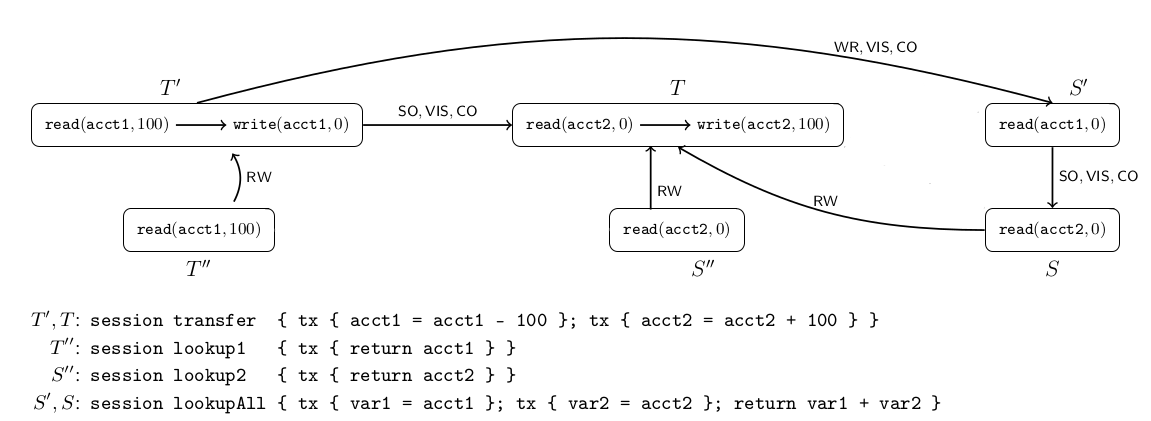
\includegraphics[scale=0.28]{fig4}
\end{figure}
The above graph is not splice-able: $\boxed{S}_\mathcal{G}$ observes write by $\boxed{T}_\mathcal{G}$ to $acct1$ but not to $acct2$.
\end{frame}

\begin{frame}
	\begin{definition}
		Given $\mathcal{G}$ let \textbf{dynamic chopping graph} $DCG(\mathcal{G})$ obtained from $\mathcal{G}$ by
		\begin{itemize}
			\item Removing $WR_\mathcal{G}, WW_\mathcal{G}, RW_\mathcal{G}$ edges between transactions related by $\approx_\mathcal{G}$
			\item Adding \textbf{predecessor} edges $SO^{-1}_\mathcal{G}$
			\item We'll call $SO$ \textbf{successor} edges
			\item And  call $\left( WR_\mathcal{G} \cup WW_\mathcal{G} \cup RW_\mathcal{G} \right) \setminus \approx_\mathcal{G}$ \textbf{conflict} edges
		\end{itemize}
	\end{definition}
\end{frame}

\begin{frame}
\begin{definition}
	A cycle in $DCG(\mathcal{G})$ is \textbf{critical} if:
	\begin{itemize}
		\item Does not contain 2 occurrences of the same vertex 
		\item Contains 3 consecutive edges in form of \textsl{conflict-predecessor-conflict}
		\item Any 2 anti dependency edges $(RW_\mathcal{G}\setminus \approx_\mathcal{G})$ are separated by at least one read $(WR_\mathcal{G}\setminus \approx_\mathcal{G})$ or write $(WW_\mathcal{G}\setminus \approx_\mathcal{G})$ dependency edge
	\end{itemize}
\end{definition}
\end{frame}


\begin{frame}
\begin{figure}
	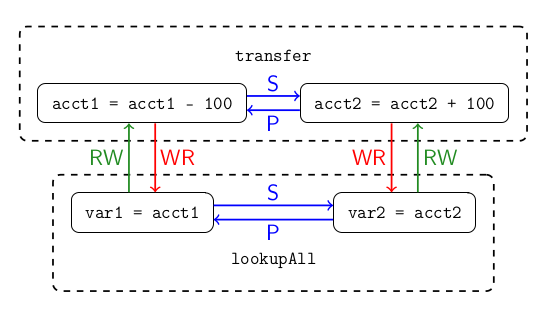
\includegraphics[scale=0.35]{fig5a}
\end{figure}
This example contains a critical cycle with $$.\xrightarrow{S}.\xrightarrow{WR}.\xrightarrow{P}.\xrightarrow{RW}.$$
\end{frame}


\begin{frame}
	\begin{theorem}
		For $\mathcal{G} \in GraphSI$, if $DCG(\mathcal{G})$ contains no critical cycles, then $\mathcal{G}$ is splice-able.
	\end{theorem}
\end{frame}


\begin{frame}
We use the last theorem to derive the static analysis.
\begin{itemize}
	\item Assume set of \textbf{programs} $\mathcal{P}=\{P_1, P_2, \dots\}$, each defining code of a session resulting from chopping a single transaction.
	\item Each $P_i$ is composed of $k_i$ \textbf{program pieces}
	\item $W^i_j$ and $R^i_j$ sets of objects written or read by j-th piece of $P_i$ 
\end{itemize}
\end{frame}

\begin{frame}
\begin{figure}
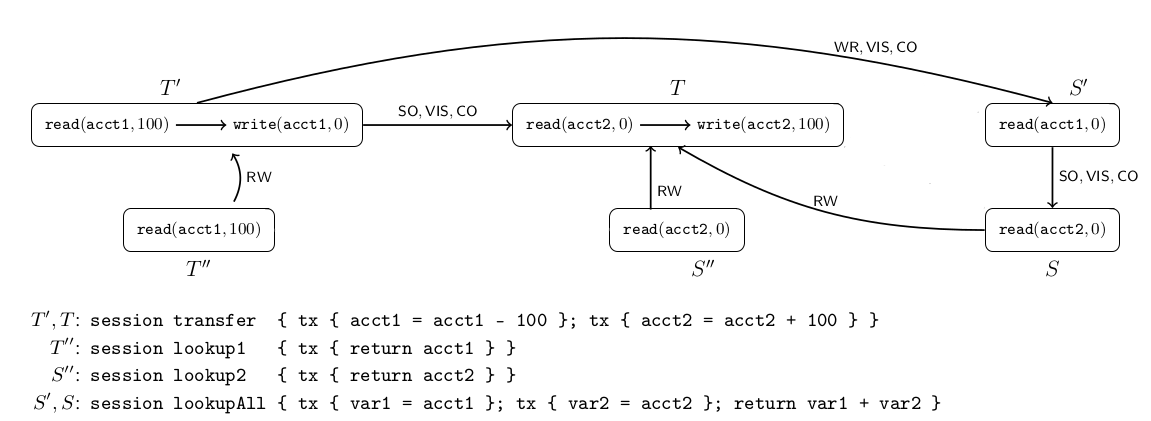
\includegraphics[scale=0.28]{fig4}
\end{figure}
For the above we have 4 \textit{programs}, one for each session. Each transaction is a \textbf{program piece}. For \texttt{transfer} session we have 2 program pieces with
\begin{itemize}
\item $W^1_1 = R^1_1 = \{acct1\}, W^1_2 = R^1_2 = \{acct2\}$
\end{itemize}
\end{frame}

\begin{frame}
	\begin{itemize}
		\item History $\mathcal{H}$ \textbf{can be produced} by programs $\mathcal{P}$ if there's 1:1 correspondence between every session in $\mathcal{H}$ and program $P_i\in\mathcal{P}$, and each transaction in the session corresponds to respective program piece, along with its read/write sets.
		\item Chopping is defined \textbf{correct} if every dependency graph $\mathcal{G}\in GraphSI$, where $\mathcal{H}_\mathcal{G}$ can be produced by $\mathcal{P}$ is splice-able.
	\end{itemize}
\end{frame}

\begin{frame}
	Consider program set $\mathcal{P}$
	\begin{definition}
		
		\textbf{Static chopping graph} $SCG(\mathcal{P})$ is a graph where nodes are program pieces in form of $(i, j)$ and the edge $(i_1, j_1), (i_2, j_2)$ is present if:
		\begin{itemize}
			\item $i_1 = i_2$ and:
			\begin{itemize}
				\item $j_1 < j_2$ (a \textbf{successor} edge)
				\item $j_1 > j_2$ (a \textbf{predecessor} edge)
			\end{itemize}
			\item $i_1 \ne i_2$ and:
			\begin{itemize}
				\item $W^{i_1}_{j_1}\cap R^{i_2}_{j_2} \ne \emptyset$ (a \textbf{read dependency} edge)
				\item $W^{i_1}_{j_1}\cap W^{i_2}_{j_2} \ne \emptyset$ (a \textbf{write dependency} edge)
				\item $R^{i_1}_{j_1}\cap W^{i_2}_{j_2} \ne \emptyset$ (an \textbf{anti dependency} edge)
			\end{itemize}
		\end{itemize}
	\end{definition}
\end{frame}

\begin{frame}
	\begin{itemize}
		\item The edge set of static graphs $SCG(\mathcal{P})$ over-approximate the edge sets of the dynamic graphs $DCG(\mathcal{G})$ corresponding to graphs $\mathcal{G}$ produced by programs $\mathcal{P}$.
		\item The chopping defined by $\mathcal{P}$ is correct if $SCG(\mathcal{P})$ contains no critical cycles (as defined for dynamic graphs).
	\end{itemize}
\end{frame}

\begin{frame}
	\begin{figure}
		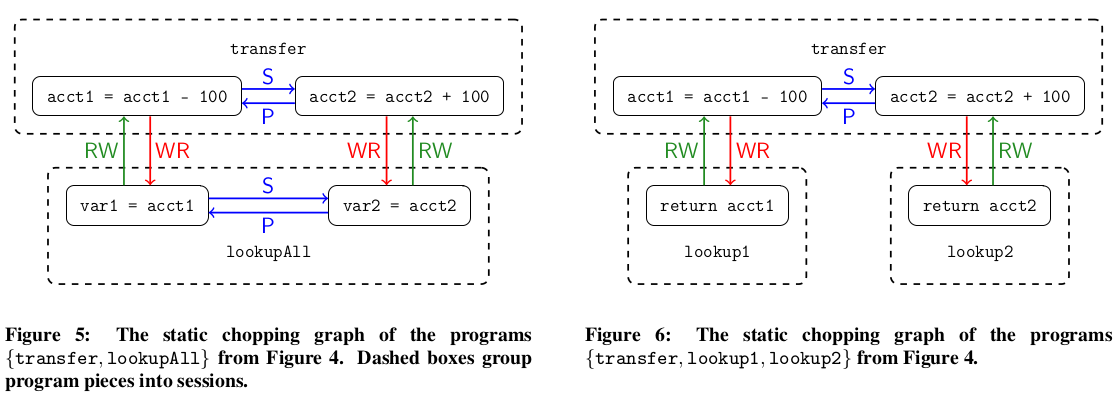
\includegraphics[scale=0.28]{fig56}
	\end{figure}
\end{frame}

\subsection{Robustness}

\begin{frame}
	\textbf{Robustness}: \\
	We'll derive an analysis that check where an application behaves the same way under a weak consistency model as it does under a strong one.
\end{frame}

\begin{frame}
	\textbf{Robustness against SI towards SER} \\
	\begin{itemize}
		\item Check if a given application running under \textbf{SI}, behaves the same as if it runs under \textbf{serializability} model.
		\item Specifically, no histories in $HistSI \setminus HistSER$
	\end{itemize}
\end{frame}

\begin{frame}
	\begin{theorem}
		For any $\mathcal{G}$, we have $\mathcal{G} \in GraphSI \setminus GraphSER $ iff. $\mathcal{T}_\mathcal{G} \vDash \textsc{Int}$, $\mathcal{G}$ contains a cycle, and all its cycles have at least two adjacent anti-dependency edges.
	\end{theorem}
\end{frame}

\begin{frame}
	Static analysis:
	\begin{itemize}
		\item Assume code of transactions defined by set of programs $\mathcal{P}$ with given read and write sets.
		\item Based on them, derive \textbf{static dependency graph}, over-approximating possible dependencies that can exist.
		\item Check that static dependency graph contains no cycles with two adjacent anti-dependency edges.
	\end{itemize}
\end{frame}


\begin{frame}
	\textbf{Robustness against PSI towards SI} \\
	\begin{itemize}
		\item Check if a given application running under \textbf{PSI}, behaves the same as if it runs under \textbf{SI} model.
		\item Again, make sure there are no histories in $HistPSI \setminus HistSI$
	\end{itemize}
\end{frame}

\begin{frame}
	\begin{definition}
		Sets of executions and histories \textbf{allowed by parallel SI} are:
		$$
		\begin{aligned}
		ExecPSI = {} &
		\begin{aligned}
			\{
				\mathcal{X} \mid
				\mathcal{X} \vDash & \textsc{Int} \wedge \textsc{Ext} \wedge \textsc{Session} \wedge \\
				& \textsc{TransVis} \wedge \textsc{NoConflict}
			\}
		\end{aligned}
		\\
		HistPSI = {} & \{ \mathcal{H} \mid \exists VIS, CO. (\mathcal{H}, VIS, CO) \in ExecPSI \}
		\end{aligned}
		$$
	\end{definition}
	\textsc{TransVis} axiom ensures that transactions ordered by $VIS$ are observed by others in this order. However, allows transactions unrelated by $VIS$ to be observed in different orders; in particular, allows \textit{long fork} anomaly.
\end{frame}

\begin{frame}
	\begin{theorem}
	Let
		\begin{multline*}
		GraphPSI = \{ \mathcal{G} \mid \left( \mathcal{T}_\mathcal{G} \vDash \textsc{Int} \right) \wedge \\
			\left(
				\left(
					\left(
					SO_\mathcal{G} \cup WR_\mathcal{G} \cup WW_\mathcal{G}
					\right)^+; RW_\mathcal{G}^?
				\right) \text{is irreflexive}
			\right)
		\}
		\end{multline*}
		Then
		\begin{multline*}
		HistPSI = \{ \mathcal{H} \mid  \exists WR,WW,RW.
		 (\mathcal{H}, WR, WW, RW) \in GraphPSI \}
		\end{multline*}
	\end{theorem}
\end{frame}

\begin{frame}
	\begin{theorem}
		For any $\mathcal{G}$, we have $\mathcal{G} \in GraphPSI \setminus GraphSI $ iff. $\mathcal{T}_\mathcal{G} \vDash \textsc{Int}$, $\mathcal{G}$ contains at least one cycle with no adjacent anti-dependency edges, and all its cycles have at least two anti dependency edges.
	\end{theorem}
\end{frame}

\begin{frame}
	FIXME example
\end{frame}

\begin{frame}
	\begin{center}
		Thank you!
	\end{center}
\end{frame}

\end{document}


